\epigraph{``And behold! When the numbers had been created for infinitely many days, the universe itself appeared. And the evening and the morning were the $\aleph$ day. And Conway looked over the rules he had made for numbers, and saw that they were very, very good. And he commanded them to be for signs, and series, and quotients, and root. Then there sprang up an infinite number less than infinity. And infinities of days brought forth multiple orders of infinities"}{Donald Ervin Knuth, Surreal Numbers \footnotemark}

\footnotetext{Excerpt of the book \textit{Surreal Numbers: how two ex-students turned on to pure mathematics and found total happiness} that precedes the moment the couple define a rule for addition of numbers.}


Conway, by counting the advantage a player has over the other in a combinatorial game, unveiled a new way to discover numbers. It is clear at this point that although numbers are not enough to represent games, they are the building blocks of all games, including the non-numbers. Until this point, the text showed some instances of the zero and hinted at 1 and -1, and the reader may also guess on how to build any integer in RB-Hackenbush and Domineering. This chapter shows that knowing that is no more than scratching the surface of surreal numbers.

For the first parts of this section a number \gam{x_1, x_2, ...}{y_1, y_2,...} might be called like a real number: $2, 5, 100000, \frac{1}{3}, \sqrt{10}, \pi$, but there is no reason believe this equality yet. There is also no reason to believe that $1 < 3$ or that 1 + 1 = 2 yet. Up until this point, numbers are labels to games that seemed to make sense. However, first a few more numbers will be labeled and only then the proofs are shown.


\subsection*{Numbers Generated in Finite Steps}

It is known that \Gm\ =
\begin{tikzpicture}
	\draw[] (0.3,-0.3) rectangle ++(0.3,0.3);
	\draw[] (0,-0.3) rectangle ++(0.3,0.3);
\end{tikzpicture} = \{ $|$ \{ $|$ \}\} = \{ $|$ 0\} was labeled $-1$.
What would be a good label for \Hm\ = 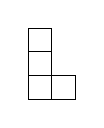
\begin{tikzpicture}
\draw[] (0.3,-0.3) rectangle ++(0.3,0.3);
\draw[] (0,-0.3) rectangle ++(0.3,0.3);
\draw[] (0,0) rectangle ++(0.3,0.3);
\draw[] (0,0.3) rectangle ++(0.3,0.3);
\end{tikzpicture}, given that it must be meaningful like described previously?\\ If it were to be labeled by a real number, which one should it be?


It is possible to find out a candidate by calculating \Gm{ + \Hm + \Hm}. To do that, one would usually find the game tree of 
\Gm{ + \Hm + \Hm}
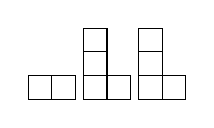
\begin{tikzpicture}
	\draw[] (-0.4,-0.3) rectangle ++(0.3,0.3);
	\draw[] (-0.7,-0.3) rectangle ++(0.3,0.3);
	\draw[] (0.3,-0.3) rectangle ++(0.3,0.3);
	\draw[] (0,-0.3) rectangle ++(0.3,0.3);
	\draw[] (0,0) rectangle ++(0.3,0.3);
	\draw[] (0,0.3) rectangle ++(0.3,0.3);
	\draw[] (1,-0.3) rectangle ++(0.3,0.3);
	\draw[] (0.7,-0.3) rectangle ++(0.3,0.3);
	\draw[] (0.7,0) rectangle ++(0.3,0.3);
	\draw[] (0.7,0.3) rectangle ++(0.3,0.3);
\end{tikzpicture}, and fill the known values bottom-up. However, it is simpler in this case. \Gm{ + 2\Hm = 0}, because whoever starts loses. Since \Gm{= -1,\,\Hm = \frac{1}{2}}. Therefore $H = \gam{{-}1, 0}{1} = \gam{0}{1} = 1/2$. The second equality is true because Left would not move to $-1$ since it is a strictly worse move than moving the game to $0$. It might not seem natural for a player to be half a move up in a game, if he/she always plays one move at a time, but it if it is desired that $\frac{1}{2} + \frac{1}{2} = 1$, that label makes sense. It might be valuable to reiterate that \Hm is definitely positive because left wins no matter who starts, but $H < 1$, as left does not have remaining move at the end of the game.

As one gets used to this area of mathematics, it becomes clear that analyzing the game \gam{1}{} is the same as analyzing 
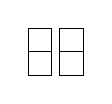
\begin{tikzpicture}
	\draw[] (0.3,-0.3) rectangle ++(0.3,0.3);
	\draw[] (0.3,0) rectangle ++(0.3,0.3);
	\draw[] (-0.1,0) rectangle ++(0.3,0.3);
	\draw[] (-0.1,-0.3) rectangle ++(0.3,0.3);
\end{tikzpicture}, but the former is not reliant on a specific game. Rather, any combinatorial game has an instance equal to \gam{1}{}. However, the rules used calculate the value of \Gm{=\gam{X}{Y}}, which are presented in the remaining of this section, help understand it better. The first practical rule in this text is finding the value of \gam{n}{} and \gam{}{{-}n}, with $n$ a natural number.

Since 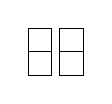
\begin{tikzpicture}
	\draw[] (0.3,-0.3) rectangle ++(0.3,0.3);
	\draw[] (0.3,0) rectangle ++(0.3,0.3);
	\draw[] (-0.1,0) rectangle ++(0.3,0.3);
	\draw[] (-0.1,-0.3) rectangle ++(0.3,0.3);
\end{tikzpicture} $= \gam{1}{}$, is it correct to assume that
$\underbrace{
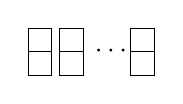
\begin{tikzpicture}
	\draw[] (1.2,-0.3) rectangle ++(0.3,0.3);
	\draw[] (1.2,0) rectangle ++(0.3,0.3);
	\draw[] (-0.1,0) rectangle ++(0.3,0.3);
	\draw[] (-0.1,-0.3) rectangle ++(0.3,0.3);
	\draw[] (0.3,0) rectangle ++(0.3,0.3);
	\draw[] (0.3,-0.3) rectangle ++(0.3,0.3);
	\node at (0.95, 0) {$\cdots$};
\end{tikzpicture}}_{n+1} = \gam{n}{}$? Yes, it is correct and the recursive nature of combinatorial games tell why. A $2\times 1$ board is equal to $1$ since Left has a move to spare. Therefore, two $2\times 1$ boards is equal to $2$ since Left has a move to spare before reaching $1$. It is simple enough to visualize it in domineering boards. The fact is it should be simple to vizualise it in any combinatorial game. A game \gam{k}{} has the same value of the sum $1+\gam{k-1}{}$ if Left's option is positive. If Left's best option is zero, then the game is equal to $1$, as already shown.

Every point discussed for \gam{X}{} is valid for \gam{}{Y}, through a similar argument.

In the last line of the proof above, the addition $(\{k-1 |\}) + 1$ was used. The notation is not the one used before, but it is possible replace $1$ with \gam{0}{}, as seems before. $\gam{k-1}{} + \gam{0}{}$ is an instance of addition described in the previous chapter. Up until this point, the integers and $\pm 1/2$ are defined. The remaining numbers fall into three categories: the multiples of powers of two, the numbers created in exactly infinite, $\aleph$, amount of steps, and the ones generated after more than infinite amount of steps. Of course the integers and 1/2 fall into the first category.

In the case of $\frac{1}{2} = \gam{0}{1}$, it is true that $G^L < G < G^R$. Is that always true? That is restricted for moves made in numbers, since in non-numbers \Gm{^R > G^L}. If left makes a move from $G$ to $G^L$, is it true that left has fewer spare moves in $G^L$ than in $G$? Before, as a side note, it was said that all possible RB-Hackenbush games are numbers, and the reason may help explain that it is true.

Suppose a game \Gm{ = \gam{X}{Y}} in which for all $x$ in $X$, $x$  is a number and for all $y$ in $Y$, $y$ is a number. Assume that $x_0$ and $y_0$ are best moves for left and right respectively. If \Gm{} is not a number, than $x_0 \ge y_0$. Now consider \Hm an instance of RB-Hackenbush. A move in \Hm corresponds to removing a colored edge from a tree and all the edges that become disconnected to the floor. Assume again for \Hm that $x_0$ and $y_0$ are edges correspondent to the best moves for left and right respectively. That means that $x_0$ is similar to  
\begin{tikzpicture}
	\draw[blue, very thick] (0,0) -- (0,0.5);
	\node at (0, 0.9) {$\vdots$};
	\node at (-0.3, 0.9) {$\ddots$};
	\node at (0.3, 0.9) {\reflectbox{$\ddots$}};
\end{tikzpicture} and $y_0$ is similar to 
\begin{tikzpicture}
	\draw[red, dash pattern=on 3pt off 0.8pt, very thick] (0,0) -- (0,0.5);
	\node at (0, 0.9) {$\vdots$};
	\node at (-0.3, 0.9) {$\ddots$};
	\node at (0.3, 0.9) {\reflectbox{$\ddots$}};
\end{tikzpicture}. Is it possible that $G^{x_i} \ge G^{y_j}$?

Consider the game built by connecting $x_0$ to the floor. The game is definitely positive, as Left wins no matter who starts. If Right starts, he/she may have an available move in a edge above the one connected to the floor. Whether it is Left playing second or first, he/she may simply remove the blue edge connected to the floor, then Right has no moves remaining and loses the game. An analogous argument shows that $y_0$ in negative. Since $x_0$ is positive, the game $\Hm^{x_0}$ resulting from removing this positive branch is less positive, or more negative, than \Hm. The same way, $\Hm^{y_0}$ is more positive or less negative that \Hm. It, in turns means that \Hm is a number.

Other phrasing for ``all RB-Hackenbush games are numbers" is ``it is not possible to make a move that improves your position in  RB-Hackenbush", or, ``left cannot make a movement that increases the value of G". Now, it may be clearer why, in numbers, $G^L < G < G^R$. A more general approach is that if neither \Gm{^L} nor \Gm{^R} have effect on the remaining moves in $G$, then it is clear that \Gm{^L} < \Gm{}. Consider the sum $\Gm{} - \Gm{^L}$. Before proceeding, the subtraction in this field means adding the negation. The negation in turns means the same game but with roles reversed. In the case of RB-Hackenbush for example, in ${-}\Gm{^L}$, Left plays the red edges.

In the sum $\Gm{} - \Gm{^L}$.

Knowing this, however, is not enough to find the value of G.

If $G = \{3 | 10\}$, it is clear that $3 < G < 10$ but what is the value of G? The \defi{simpler} number that fits the interval, 4. There are some equivalent ways to check which number is simpler. A good one is figuring out which one require less effort to write in their recursive and simplified form. For example, the simplified, recursive form for 4 is $\{\{\{\{\{|\}|\}|\}|\} | \}$. Another good way is deciding which one is younger in the number tree represented below.

It is very recommended to understand that the \defi{simplicity principle} is indeed finding the simplest number from a range of possibilities. An integer with smallest modulo is simple than one with greater modulo, and an irreducible fraction with denominator 2 is simpler than one with denominator 4. The formula for the simplicity principle, however, is 

G = 
$
\begin{cases}
	0, &\text{if } G^L < 0 < G^R\\
	n+1, &\text{if } \Gm{= \gam{n}{}}\\
	-n-1, &\text{if } \Gm{= \gam{}{{-}n}}\\
	\frac{2p + 1}{2^{q+1}}, &\text{if } \Gm{= \gam{\frac{p}{2^q}}{ \frac{p+1}{2^q}}}
\end{cases}
$

\vspace{0.6em}Some examples are $\frac{1}{4} =$ \gam{0.1}{0.3}, $\frac{1}{8} =$ \gam{\frac{1}{9}}{0.2}, $\frac{-3}{4} =$ \gam{-1}{{-}0.6}.

\subsection*{Numbers Generated After Infinite or More Steps}

The formula above only allows \Gm{} to have an infinite amount of values, but it is not closes to what was stated in the beginning of the section. The remaining numbers are hidden in the end of infinite games, in the sense that the board size is infinite, because, as explained before, it is extremely unpleasant to play something that does not end. 

\begin{figure} [!ht]
\begin{center}
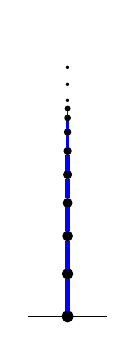
\begin{tikzpicture}
	\begin{scope} [every node/.style={scale=0.3, style=circle, draw, fill=black}]
		\node [scale=1.4] (1) at (0, -1.80){};
		\node [scale=1.3] (2) at (0, -1.26){};
		\node [scale=1.2] (3) at (0, -0.78){};
		\node [scale=1.1] (4) at (0, -0.36){};
		\node [scale=1]   (5) at (0, 0)      {};
		\node [scale=0.9] (6) at (0, 0.3)  {};
		\node [scale=0.8] (7) at (0, 0.54) {};
		\node [scale=0.7] (8) at (0, 0.72) {};
		\node [scale=0.6] (9) at (0, 0.84) {};
		\node [scale=0.2, fill=white, draw=none] at (0, 1.1) {$\vdots$};
	\end{scope}
	\draw (-0.5,-1.80) -- (0.5, -1.80);
	\draw[blue, ultra thick] (1)--(2);
	\draw[blue, ultra thick] (2)--(3);
	\draw[blue, ultra thick] (3)--(4);
	\draw[blue, ultra thick] (4)--(5);
	\draw[blue, ultra thick] (5)--(6);
	\draw[blue, thick] (6)--(7);
	\draw[blue, thick] (7)--(8);
	\draw[blue] (8)--(9);
	\node[scale=1.5] at (0, 1.3) {\scriptsize$\vdots$};
\end{tikzpicture}
\end{center}
\end{figure}

In the game above, left has an infinite number of possible moves, but \todo{his/her} move always leads to an integer. What is the value of this game? \gam{1,2,...}{}, It happens that this number has been baptized much earlier in mathematics of $\omega$, the first ordinal number. It might not be as straight forward as finitely generated numbers, but the principle to calculate the value is the same.

For any finite number of red edges in \Gm{}, if you add the game above to \Gm{}, the result will be positive. However, it is also very simple to verify that $\omega$ is by far not the largest possible advantage. One simple  example of that is the following.

\begin{figure} [!ht]
\begin{center}
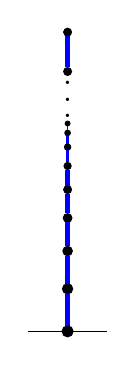
\begin{tikzpicture}
	\begin{scope} [every node/.style={scale=0.3, style=circle, draw, fill=black}]
		\node [scale=1.4] (1) at (0, -1.80){};
		\node [scale=1.3] (2) at (0, -1.26){};
		\node [scale=1.2] (3) at (0, -0.78){};
		\node [scale=1.1] (4) at (0, -0.36){};
		\node [scale=1]   (5) at (0, 0)      {};
		\node [scale=0.9] (6) at (0, 0.3)  {};
		\node [scale=0.8] (7) at (0, 0.54) {};
		\node [scale=0.7] (8) at (0, 0.72) {};
		\node [scale=0.6] (9) at (0, 0.84) {};
		\node [scale=0.2, fill=white, draw=none] at (0, 1.1) {$\vdots$};
		\node [scale=1] (10) at (0, 1.5) {};
		\node [scale=1] (11) at (0, 2) {};
	\end{scope}
	\draw (-0.5,-1.80) -- (0.5, -1.80);
	\draw[blue, ultra thick] (1)--(2);
	\draw[blue, ultra thick] (2)--(3);
	\draw[blue, ultra thick] (3)--(4);
	\draw[blue, ultra thick] (4)--(5);
	\draw[blue, ultra thick] (5)--(6);
	\draw[blue, thick] (6)--(7);
	\draw[blue, thick] (7)--(8);
	\draw[blue] (8)--(9);
	\node[scale=1.5] at (0, 1.3) {\scriptsize$\vdots$};
	\draw[blue, ultra thick] (10)--(11);
\end{tikzpicture}
\end{center}
\end{figure}

The game above is an infinite stack of blue edges with another one on the top. One could wrongly argue that this additional edge on the top is simply part of the infinite stack. This is a wrong argument because this additional edge on the top allows Left to move to $\omega$, and therefore, has the value of $\omega+1$, making the games different. This detail is paramount to understanding the statement found on the epigraph of this section.

A hypothetical John Horton Conway wrote that phrase near a cave close to the edge of the Indian Ocean, where a couple of future mathematicians went to find themselves. The words attributed to Conway by Knuth say that in the $\aleph$th day the universe appeared. That is because Knuth realizes that in that specific days all real numbers are generated.

However, again, accordingly to the hypothetical Conway, days kept passing by and more numbers were generated. The number $\omega+1$ is one of the infinitely many surreal numbers that are not real numbers. However, this is not in the slightest the end of story. In fact, even considering that $\omega + \omega + ...$  is also generated in the same format, the important part might again be missed. That is because only looking at large numbers is not way forward.

As seem before $\frac{1}{2} = \gam{0}{1}, \frac{1}{4} = \gam{0}{\frac{1}{2}}, \cdots, \frac{1}{2^{n+1}} = \gam{0}{\frac{1}{2^n}}$. Therefore, the same way that $\omega=\gam{1,2,...}{}$, $\epsilon=\gam{0}{1,\frac{1}{2},\frac{1}{4},\cdots}$. A game with value $\epsilon$ may be simply the game of RB-Hackenbush starting with a blue edge and following with an infinite number of red edges. First notice that $\epsilon$ still have positivity, because Left wins no matter who starts, and then notice that its positivity is smaller than that of any real number. Now that $\epsilon$ and $\omega$ are known members of the $\aleph$ day, only the remaining real numbers remain.

The fact that real numbers are generated in the $\aleph$th day and how to generate them with possible games is part of the section 5. The reason for that is that although it is easy generating reals with RB-Hackenbush games, it might also be worth it to know how to generate them with other games, and in fact, any other games.

\subsection*{The Surreal Numbers}

This text presents only few characteristics of the surreal numbers as they are not the focus. It is also not necessary to know every algebraic property of numbers to go forward with the study of temperature this text focus on. However, it so happens that with very few construction rules, the numbers contain all the real, ordinal and infinitesimal numbers.

Because of its extremely simple definition and big expressiveness, it is an extremely interesting topic. The idea that the number os spare moves a player has might not be a real number might not be confusing, but it should be somewhat hard to accept. It is true that this fact is based on the construction Conway made and it is not necessarily true for all ways to analyze games, but the straight forward way of using game trees to build numbers lead to this characteristic.

Because the creation/discovery of surreals is very recent, it definitely makes people apprehensive as it is not clear if its properties are good or bad. The mathematician Phillip Ehrlich is an eloquent participant in this discussion. He makes the point that the surreals do not have an intrinsic problem and that they show an unifying nature between paths in mathematics. In one of his papers, Ehrlich proposes that, while the real numbers form, on his words, an arithmetic continuum, the surreals form the absolute arithmetic continuum.

However, it is still a problem converting the domain of typical studies, such as calculus, from the reals to the surreals. Integrals of functions in the surreals are particularly hard to define. The 2015 revision of the paper ANALYSIS ON SURREAL NUMBERS, by SIMON RUBINSTEIN-SALZEDO AND ASHVIN SWAMINATHAN, for example, gave a definition of integration that solved a problem with previous integration but it is clear that others persist.

As Salzedo and Swaminathan point-out: ``The `Conway-Norton'\footnote{In ONAG 2nd edition page 228, Conway  tells that Norton's definition of integrals do not have desired properties.}
integral failed to have standard properties of real integration, however, such as translation
invariance: $\int_a^bf(x)dx = \int_{a-t}^{b-t}f(x+t)dx$, for any surreal function f and $a,b,t\in$ \textbf{No}. While Fornasiero fixed this issue in [For04]\footnote{Antongiulio Fornasiero Phd. Thesis: \textit{Integration on surreal numbers.}}, the new integral, like its predecessor, yields
$exp(\omega)$ instead of the desired $exp(\omega)-1$ for $\int_0^{\omega}exp(x)dx$". In the ``Open Questions" section of  the paper, the authors tell that there are still problems with their definition, meaning that the conversion of domains in integral studies is not completed, at least by 2015.

While many questions remain open, however, it is still possible to work with a subset of the surreals that only contain the reals for example. The remaining of the text does not require profound knowledge of anything that is not mentioned in regards to numbers.









